\documentclass[tikz,border=10pt]{standalone}
\usetikzlibrary{calc}
\begin{document}
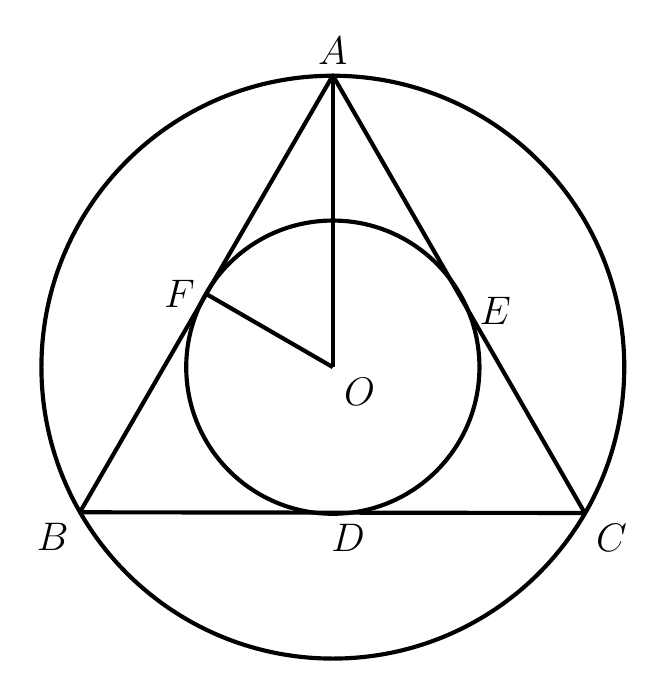
\begin{tikzpicture}[line width=1.5pt, line join=round]
% Scale s = 0.018824 cm/px (from STYLE METRICS), y axis flipped about O(239,261.7)
\coordinate (O) at (0,0);
\coordinate (A) at (0,3.705);
\coordinate (B) at (-3.213,-1.843);
\coordinate (C) at (3.200,-1.852);
\coordinate (D) at (0.194,-1.850);
\coordinate (E) at (1.721,0.715);
\coordinate (F) at (-1.608,0.930);

% circumcircle and incircle, both centred at O
\draw (O) circle (3.701);
\draw (O) circle (1.862);

% triangle ABC
\draw (A) -- (B) -- (C) -- cycle;

% segment AO (vertical)
\draw (A) -- (O);

% segment OF (F lies on AB)
\draw (O) -- (F);

% labels
\node[above, font=\fontsize{15.5}{18.6}\selectfont] at (A) {$A$};
\node[below left, font=\fontsize{15.5}{18.6}\selectfont] at (B) {$B$};
\node[below right, font=\fontsize{15.5}{18.6}\selectfont] at (C) {$C$};
\node[below, font=\fontsize{15.5}{18.6}\selectfont] at (D) {$D$};
\node[right, font=\fontsize{15.5}{18.6}\selectfont] at (E) {$E$};
\node[left, font=\fontsize{15.5}{18.6}\selectfont] at (F) {$F$};
\node[below right, font=\fontsize{15.5}{18.6}\selectfont] at (O) {$O$};
\end{tikzpicture}
\end{document}